% time values for run2/10, run4/11, run15/16
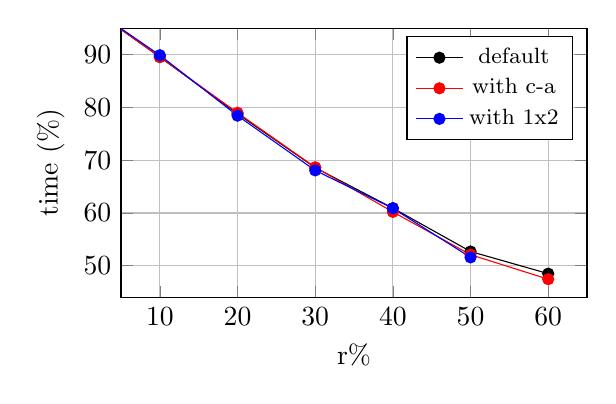
\begin{tikzpicture}
\begin{axis}[
    title={},
    height=5cm,
    width=7.5cm,
    xlabel={r\%},
    ylabel={time (\%)},
    xmin=5, xmax=65,
    ymin=44, ymax=95,
    xtick={10,20,30,40,50,60},
    ytick={50,60,70,80,90},
    legend pos=north east,
    xmajorgrids=true,
    ymajorgrids=true,
    legend style={font=\footnotesize}
]

\addplot[
    color=black,
    mark=*
    ]
    coordinates {
    (0,100)(10,89.54)(20,78.79)(30,68.58)(40,60.91)(50,52.70)(60,48.50)
    };
    
\addplot[
    color=red,
    mark=*
    ]
    coordinates {
    (0,100)(10,89.54)(20,78.98)(30,68.65)(40,60.20)(50,52.09)(60,47.45)
    };

\addplot[
    color=blue,
    mark=*
    ]
    coordinates {
    (0,100)(10,89.89)(20,78.43)(30,68.06)(40,60.88)(50,51.58)
    };
    
\legend{default, with c-a, with 1x2}
    
\end{axis}
\end{tikzpicture}